The system is divided in the following subsystems:
\begin{itemize}
    \item Web application
    \item Mobile application
    \item Customer mobile services
    \item Employee web services
    \item Store manager web services
    \item Queue manager
    \item Visit scheduler
    \item External subsystems like: Maps APis, OS Notif. Gateway and DBMS
\end{itemize}
As said in the section 2.2, \textit{Web application} and \textit{Mobile application} compose the client-side of our system, \textit{Customer mobile services}, \textit{Employee mobile services} and \textit{Store manager web services} compose the server-side business logic of our system, together with \textit{Queue manager} and \textit{Visit scheduler}. 

The listed subsystems have to be implemented, tested, and integrated using a bottom-up approach. To do so, we provide a development order based on the dependencies to make possible a step-by-step implementation and components integration testing (respecting the technique of the bottom-up approach). To accelerate the development process, we opted for a mixed process, where there are macro-phases (implementation, unit testing, and integration testing) to be completed before others. As for the two sides: client-side and server-side, this can be developed in parallel, they will be integrated and tested together in the final integration part.

It should be noted that it is not considered necessary to implement the external components mentioned above as they are assumed to be external and reliable.

The following table presents the development stages with which we summarize the various steps of the development process and the execution order. For each step, a forecast of development difficulties has also been noted.

\begin{center}
    {\renewcommand{\arraystretch}{2}%
    \begin{tabular}{C{3cm}L{6cm}L{4cm}}
        \hline
        \textbf{Order number} & \textbf{Development stage} & \textbf{Development difficult} \\
        \hline
        1 & Store Manager and Customers Sign up and Log in Developing & Low \\
        \hline
        2 & Employee Registration by Store Manager Developing & Low \\
        \hline
        3 & Employee Login Developing & Low \\
        \hline
        4 & Visit Scheduling Business Logic Developing & Medium \\
        \hline
        5 & Book a Visit Developing & Medium \\
        \hline
        6 & Queue Business Logic Developing & Medium \\
        \hline
        7 & Employee and Customer Line Up Reservation Developing & High \\
        \hline
        8 & Entrances and Exits Developing & Low \\
        \hline
        9 & Data Analyzer Developing & Medium \\
        \hline
        10 & Statistics and Data Elaborator Developing & Low \\
        \hline
        11 & Client-Side and Server-Side Integration & \\
        \hline
    \end{tabular}}
\end{center}

    \subsection{Development Stages Definition}
    In the following enumeration, we specify for each stage, what components are implemented in the stage, and how the components are integrated and tested (there is an integration diagram for each stage).        
    \begin{enumerate}
            \item \textbf{Store Manager and Customers Sign up and Log in Developing}: In this step it's necessary to implement and produce unit test for the \textit{AccountManager} component (Store Manager Web Services, Customer Mobile Services). This modules are the first two to be developed following a bottom-up approach, they communicates with the DBMS (external reliable component). We choose this as first step because some components need features developed in this stage (like store information about the actors) \begin{figure}[H]
                \centering
                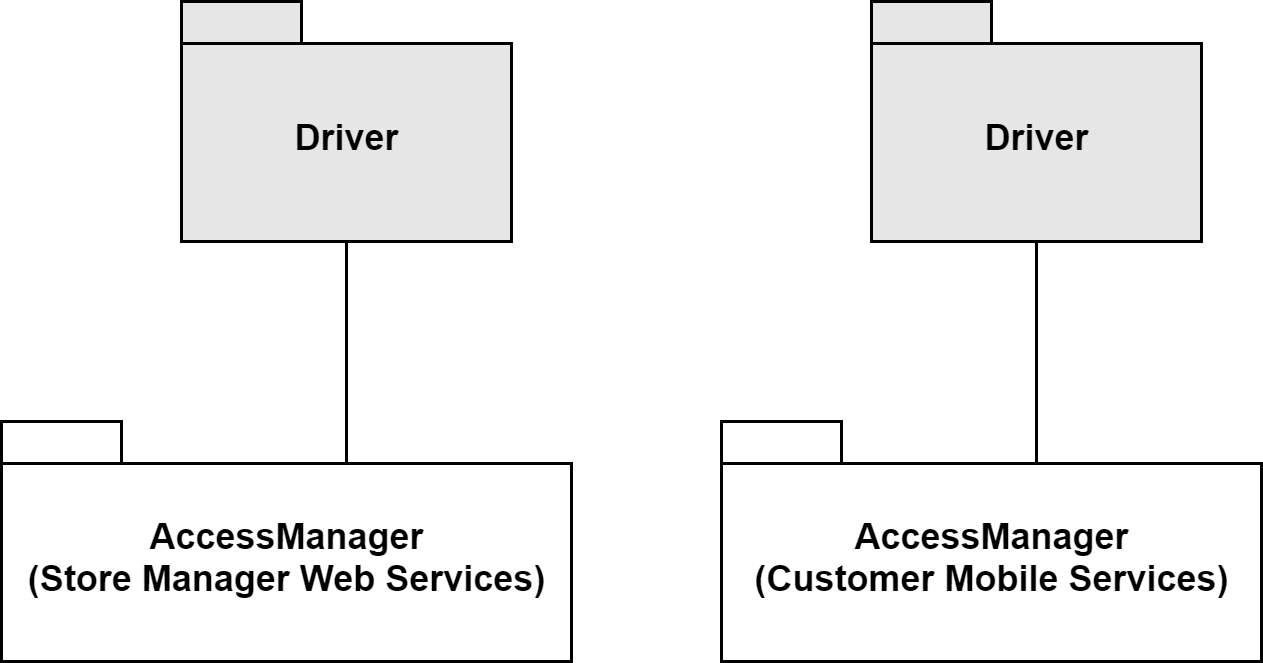
\includegraphics[width=6cm]{int_diagr1.png}
            \end{figure}
            \item \textbf{Employee Registration by Store Manager Developing}: In this step it's necessary to implement and produce unit test for the component \textit{StoreInfoAndEmployeeManager}. As you can see in the diagram, the component developed has to be integrated and tested with \textit{AccessManager}. Following the bottom-up approach it uses a Driver to represents the high level components to be developed  \begin{figure}[H]
                \centering
                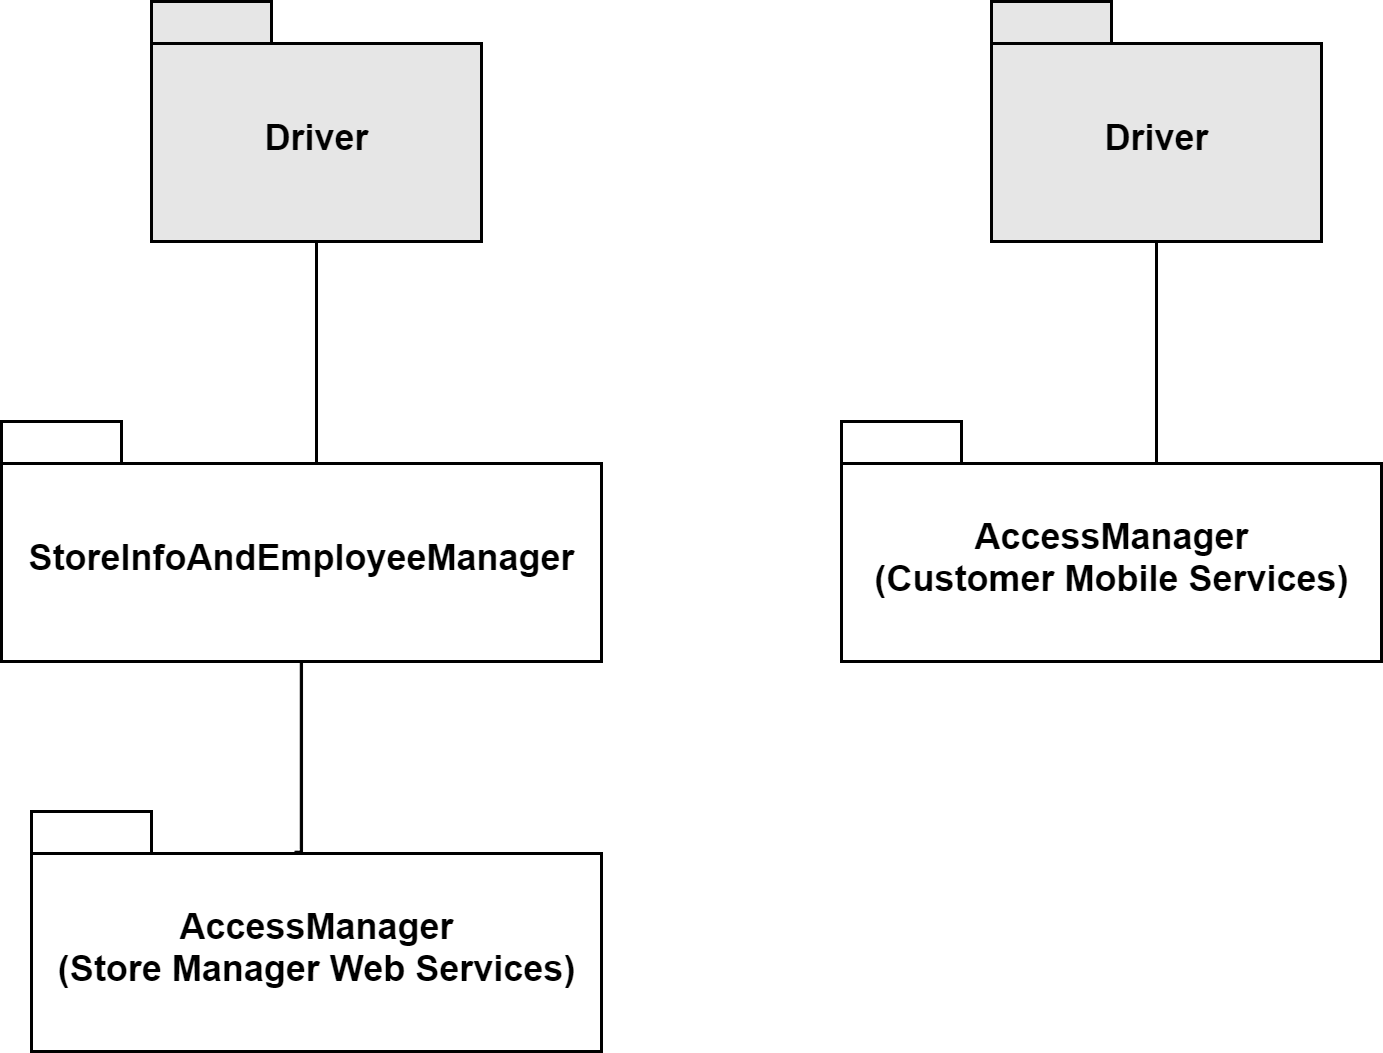
\includegraphics[width=6cm]{int_diagr2.png}
            \end{figure}
            \item \textbf{Employee Login Developing}: In this step it's necessary to implement and produce unit test for the component \textit{AccessManager} (Employee Web Services). As you can see in the diagram, the component developed has to be integrated and tested with \textit{StoreInfoAndEmployeeManager}. Following the bottom-up approach it uses a Driver to represents the high level components to be developed \begin{figure}[H]
                \centering
                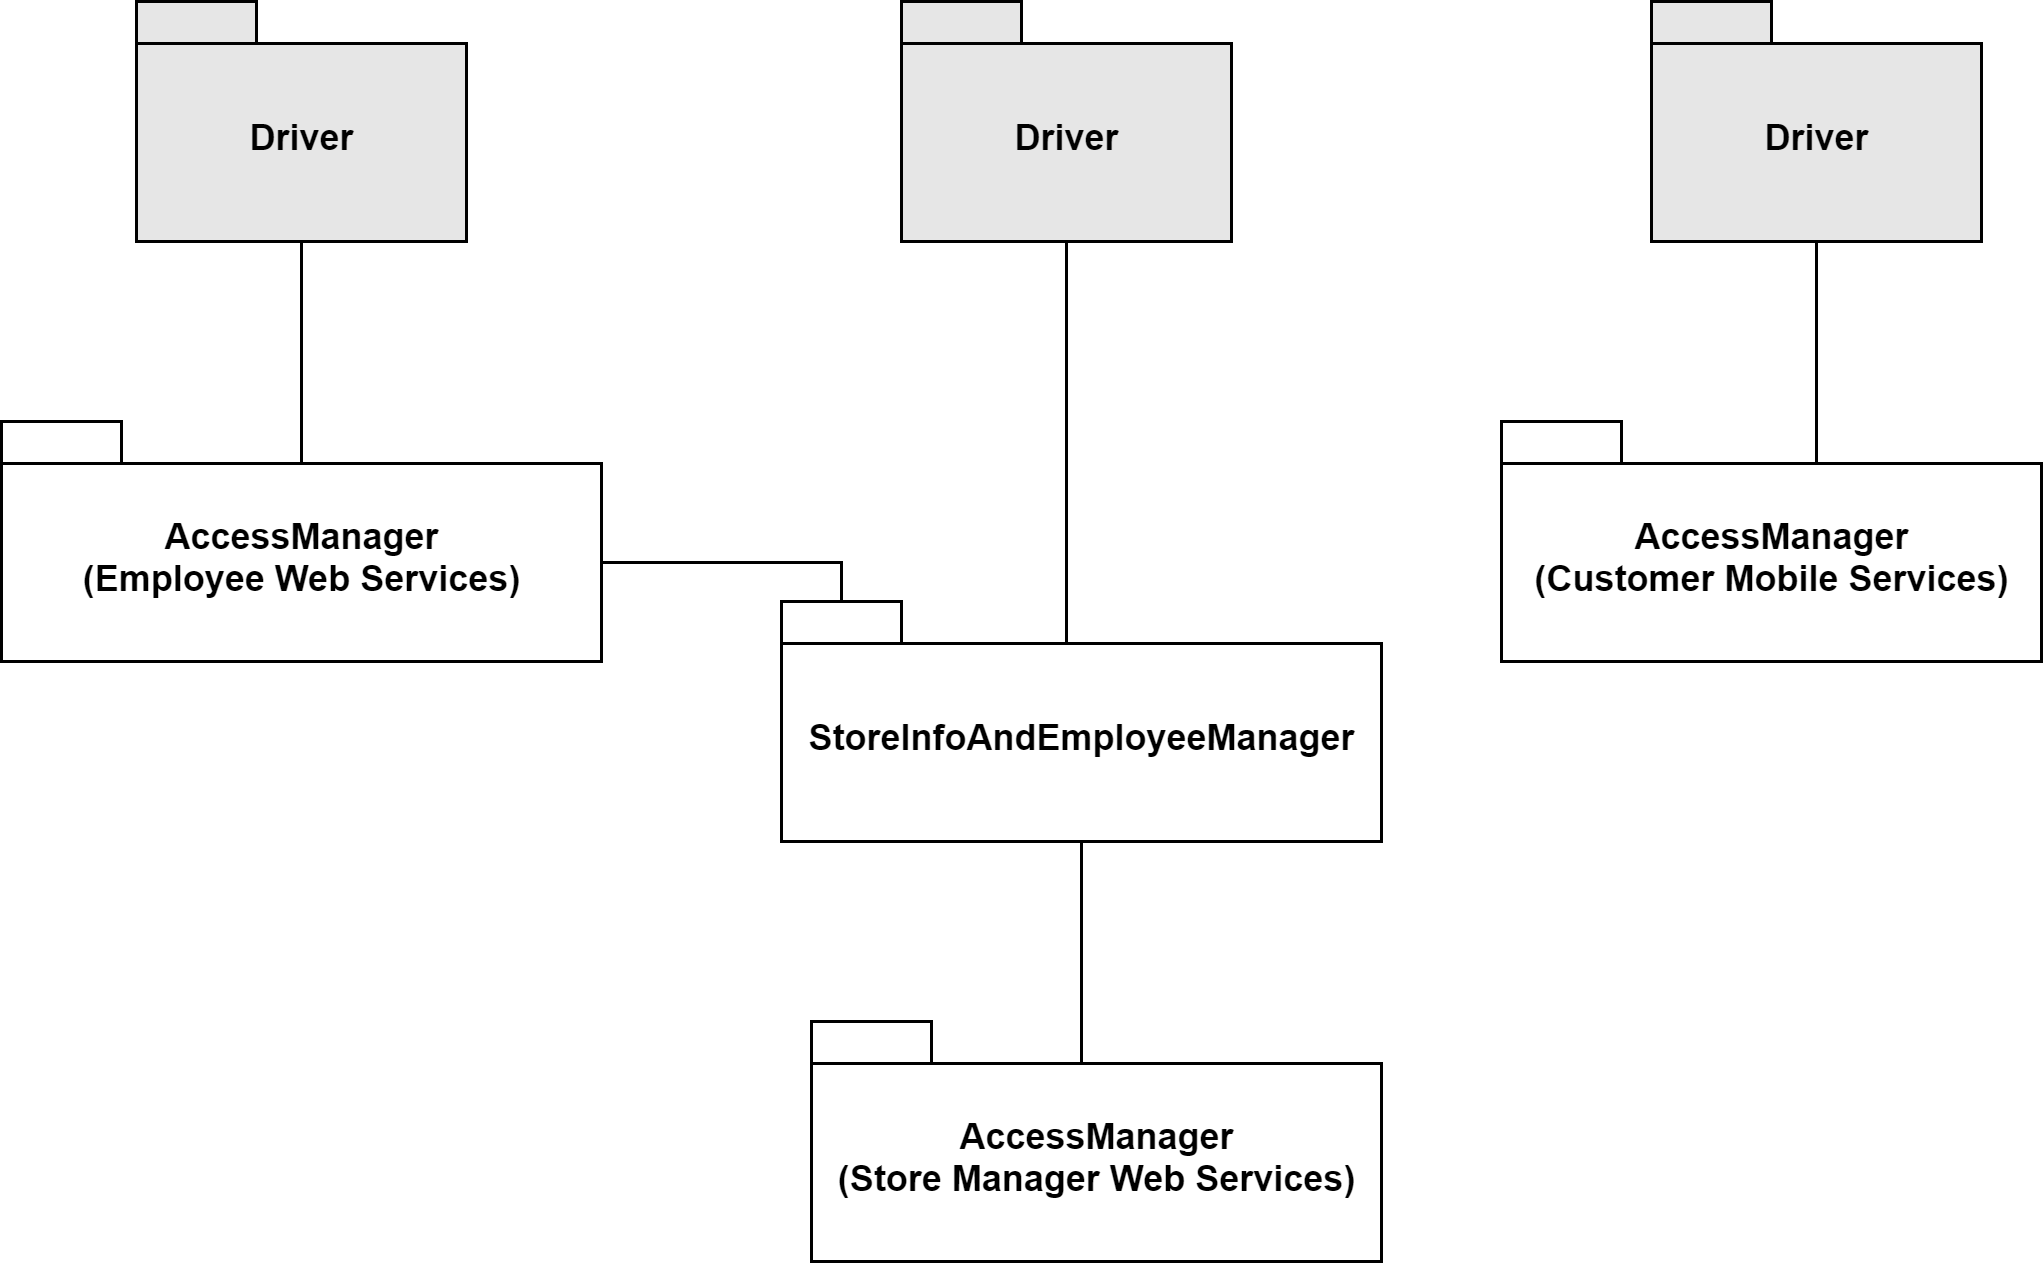
\includegraphics[width=8cm]{int_diagr3.png}
            \end{figure}
            \item \textbf{Visit Scheduling Business Logic Developing}: In this step it's necessary to implement and produce unit test for the component \textit{VisitScheduler}. As you can see in the diagram, the component in this stage hasn't to be integrated and tested with other components but, following the bottom-up approach it uses a Driver to represents the high level components to be developed \begin{figure}[H]
                \centering
                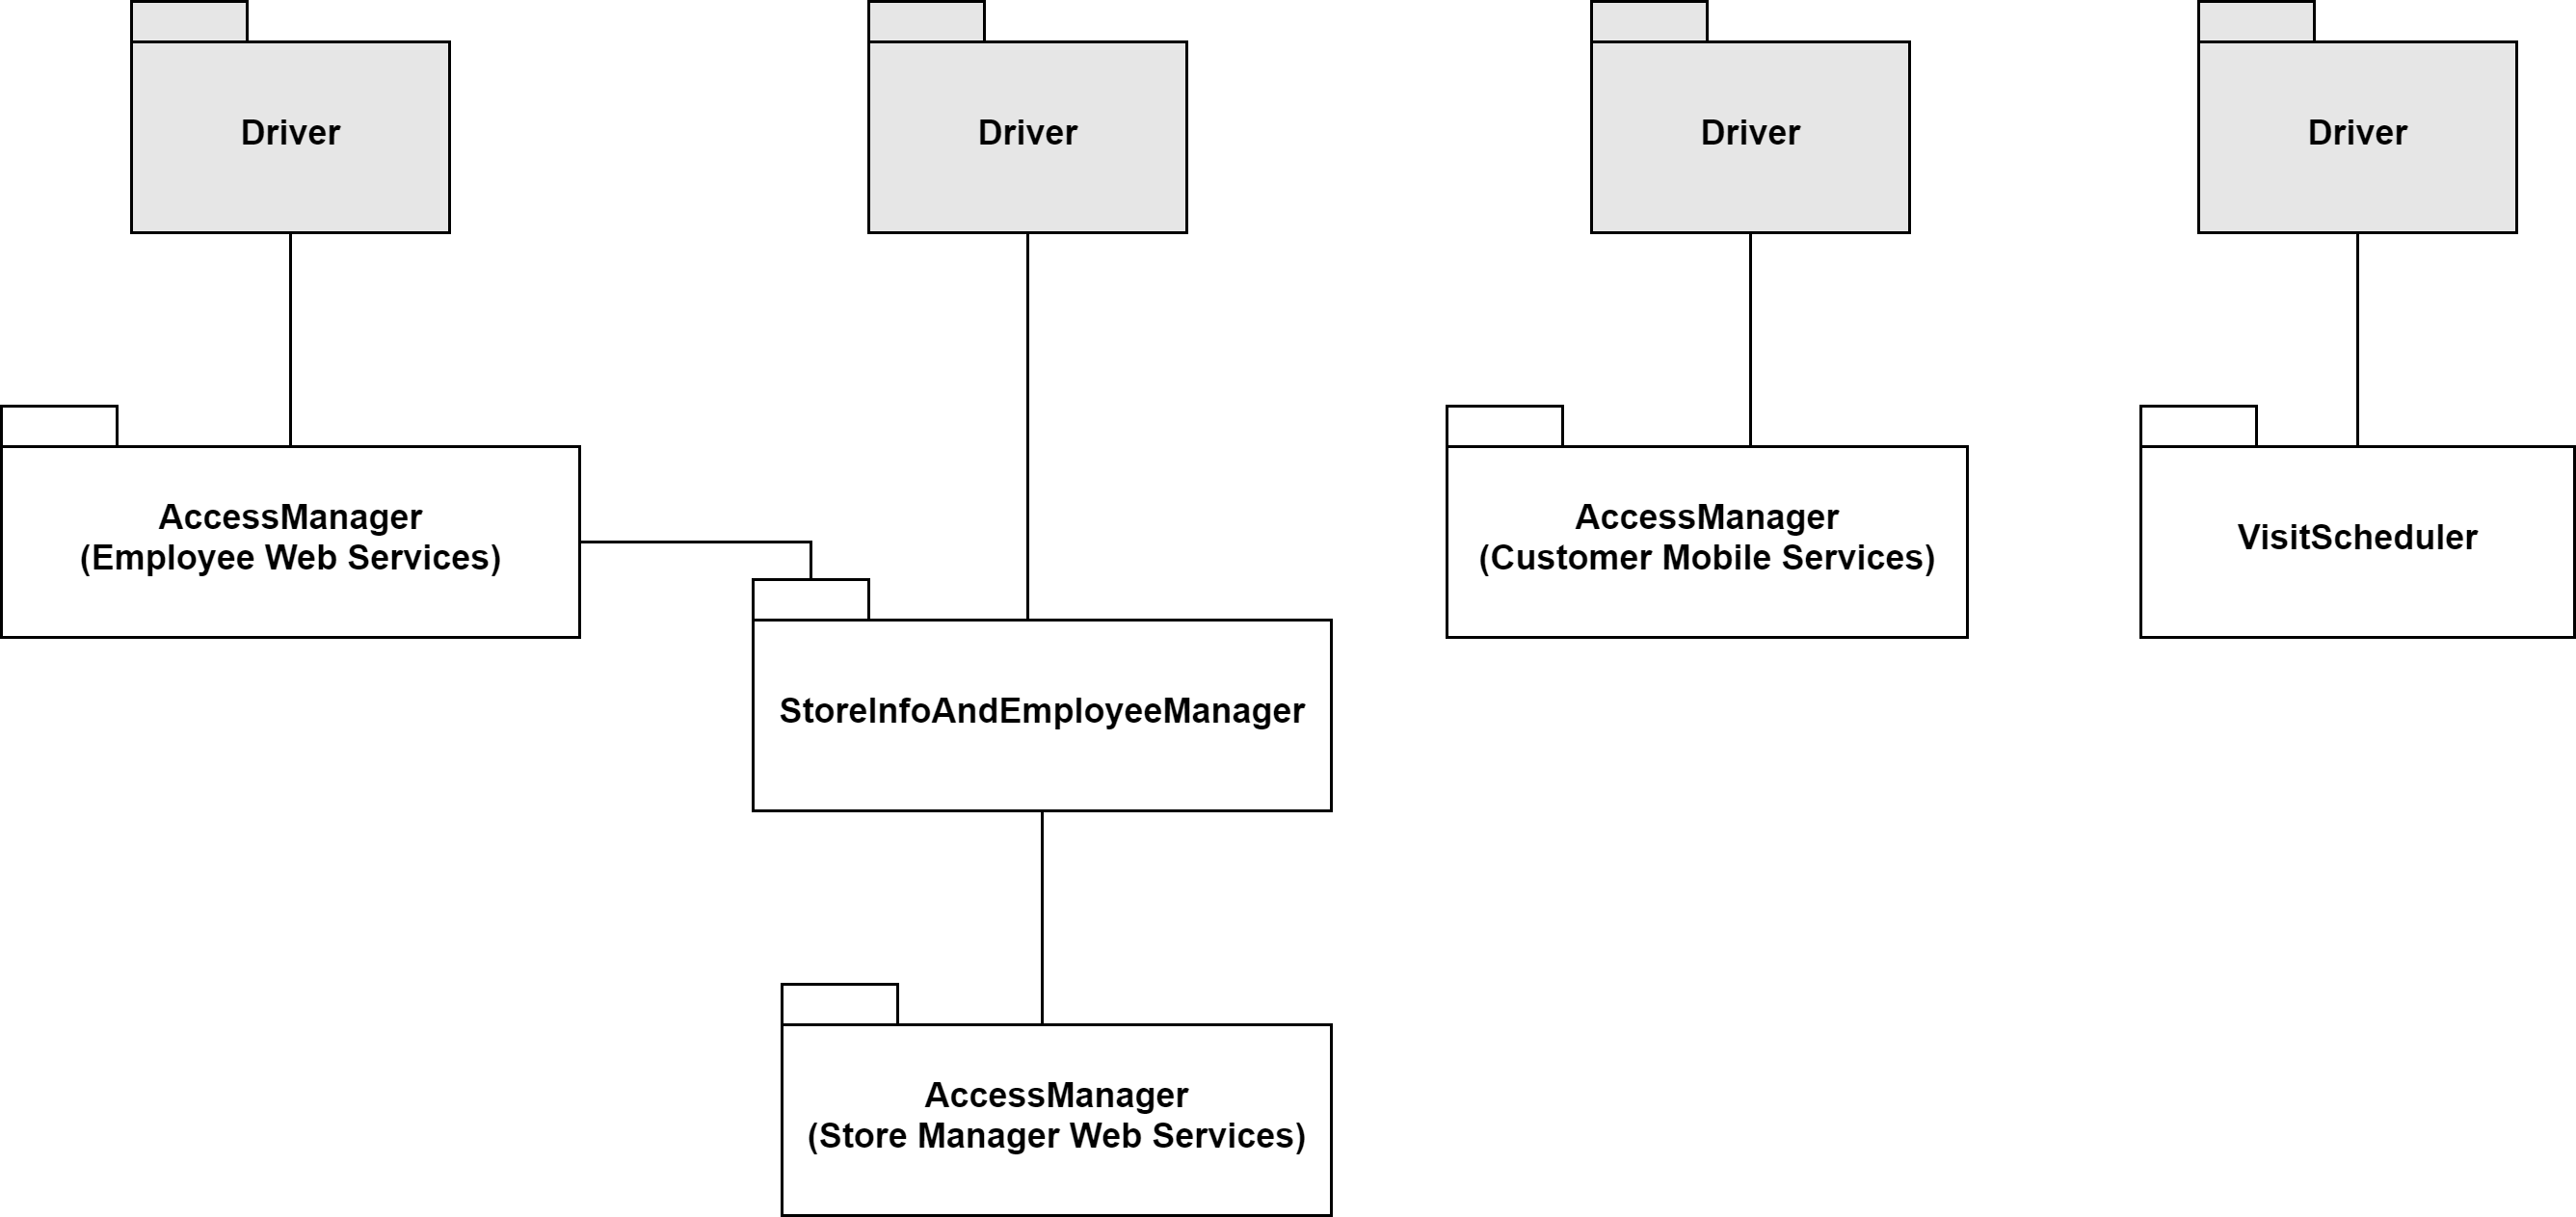
\includegraphics[width=10cm]{int_diagr4.png}
            \end{figure}
            \item \textbf{Book a Visit Developing}: In this step it's necessary to implement and produce unit test for the component \textit{VisitReservationModule}. As you can see in the diagram, the component in this stage has to be integrated and tested with \textit{VisitScheduler} and \textit{AccessManager}. Following the bottom-up approach it uses a Driver to represents the high level components to be developed \begin{figure}[H]
                \centering
                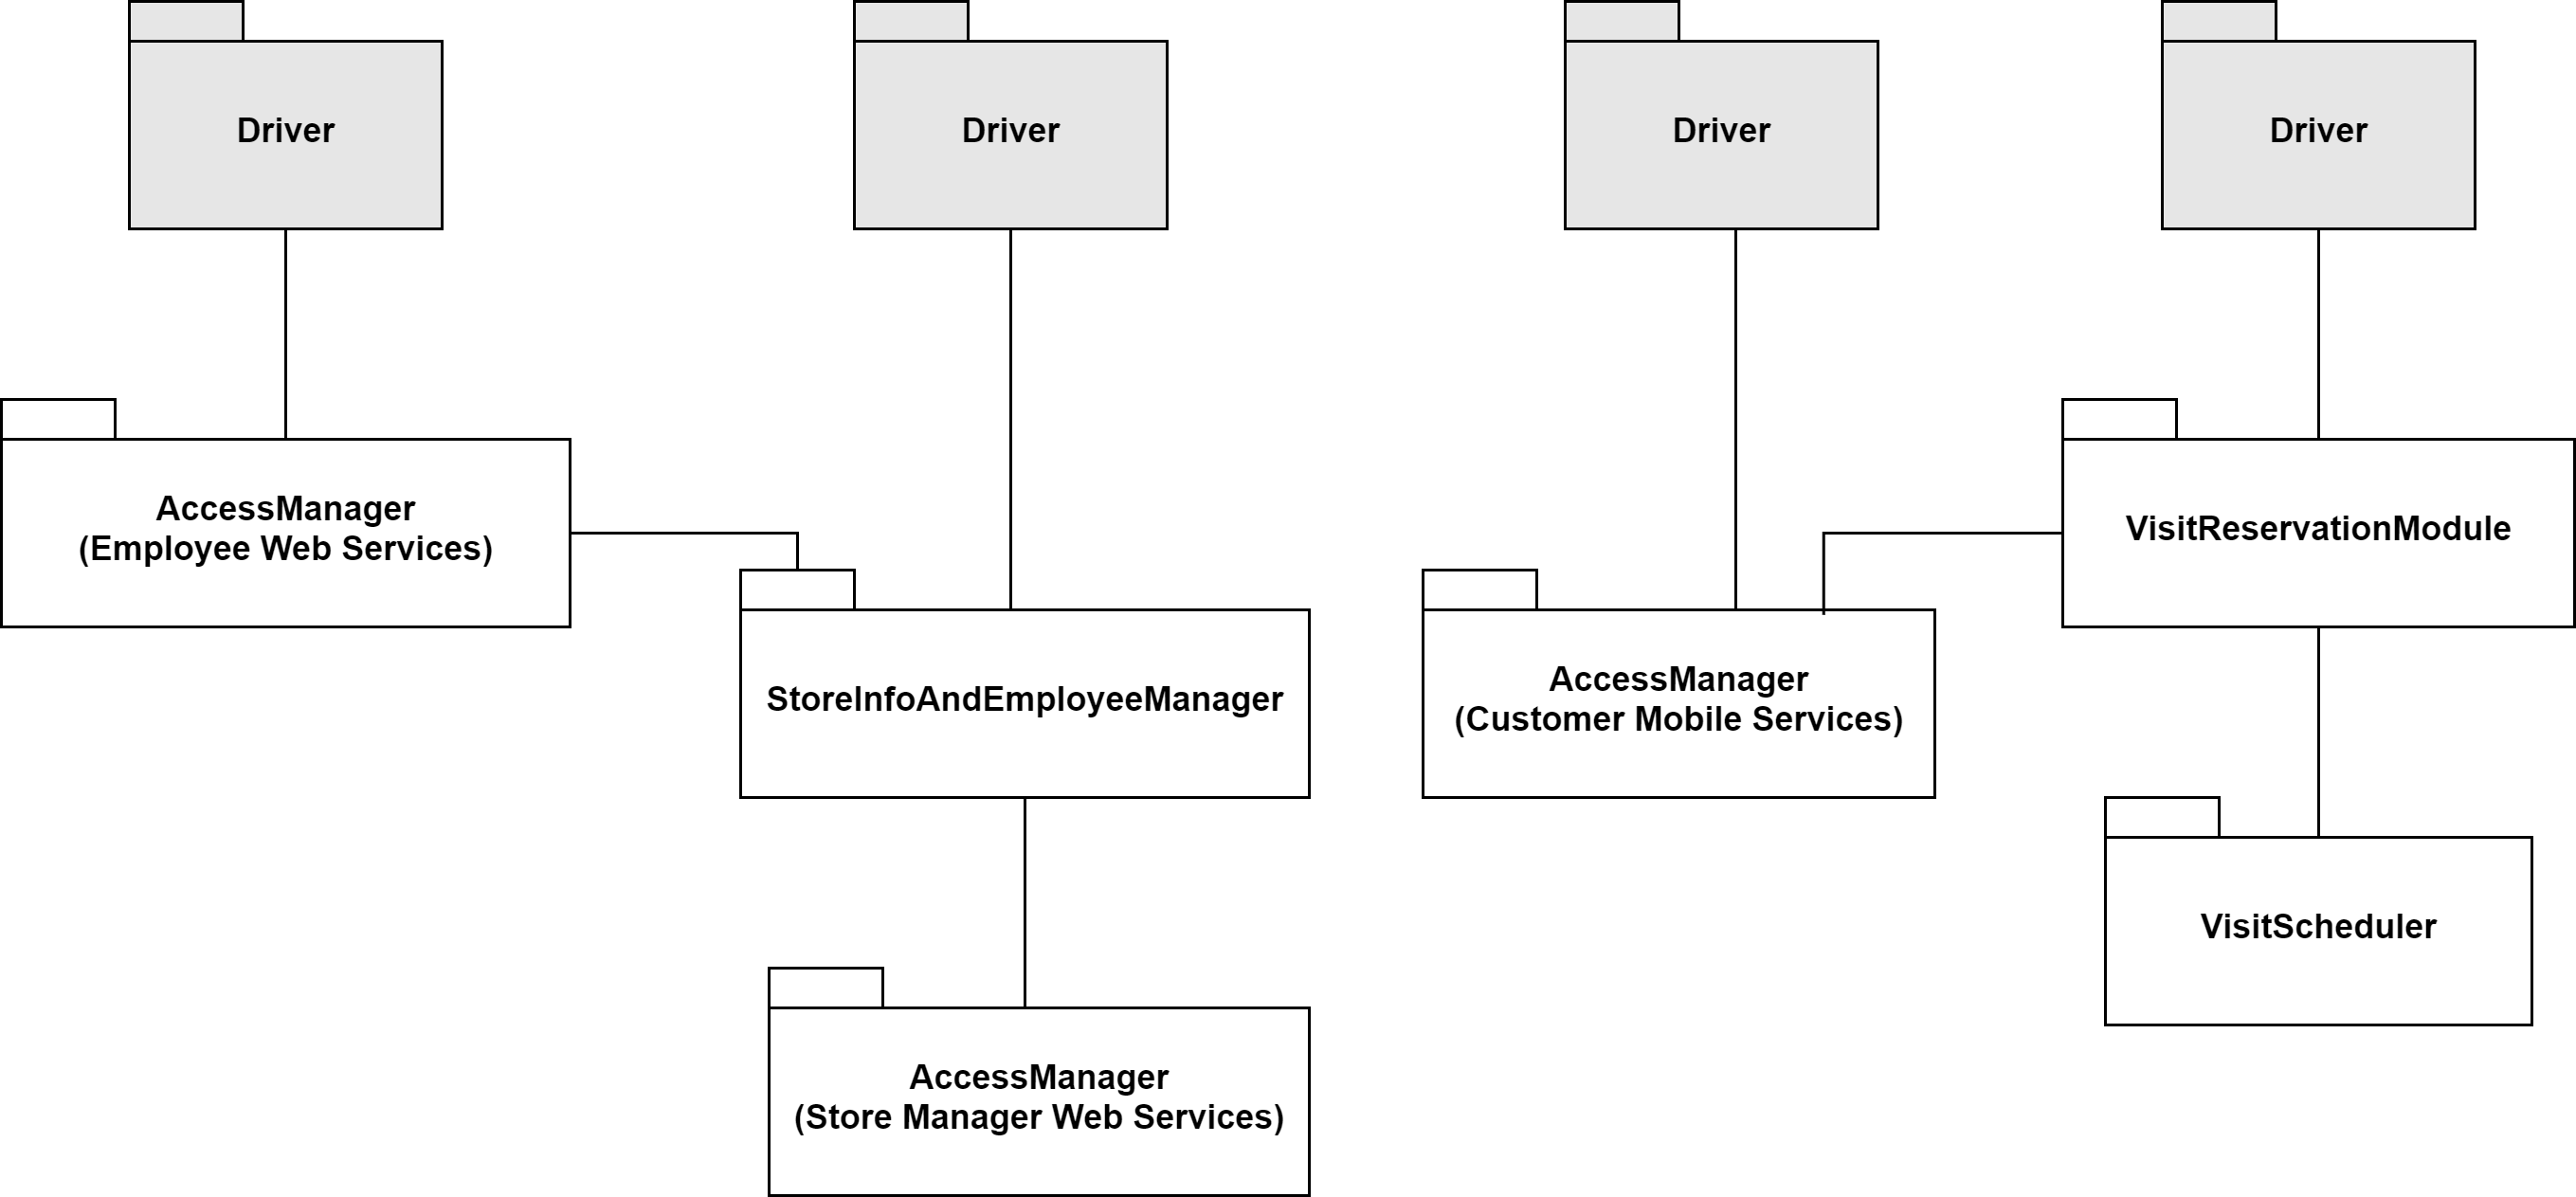
\includegraphics[width=10cm]{int_diagr5.png}
            \end{figure}
            \item \textbf{Queue Business Logic Developing}: In this step it's necessary to implement and produce unit test for the component \textit{QueueManager}. As you can see in the diagram, the component in this stage hasn't to be integrated and tested with other components. Following the bottom-up approach it uses a Driver to represents the high level components to be developed \begin{figure}[H]
                \centering
                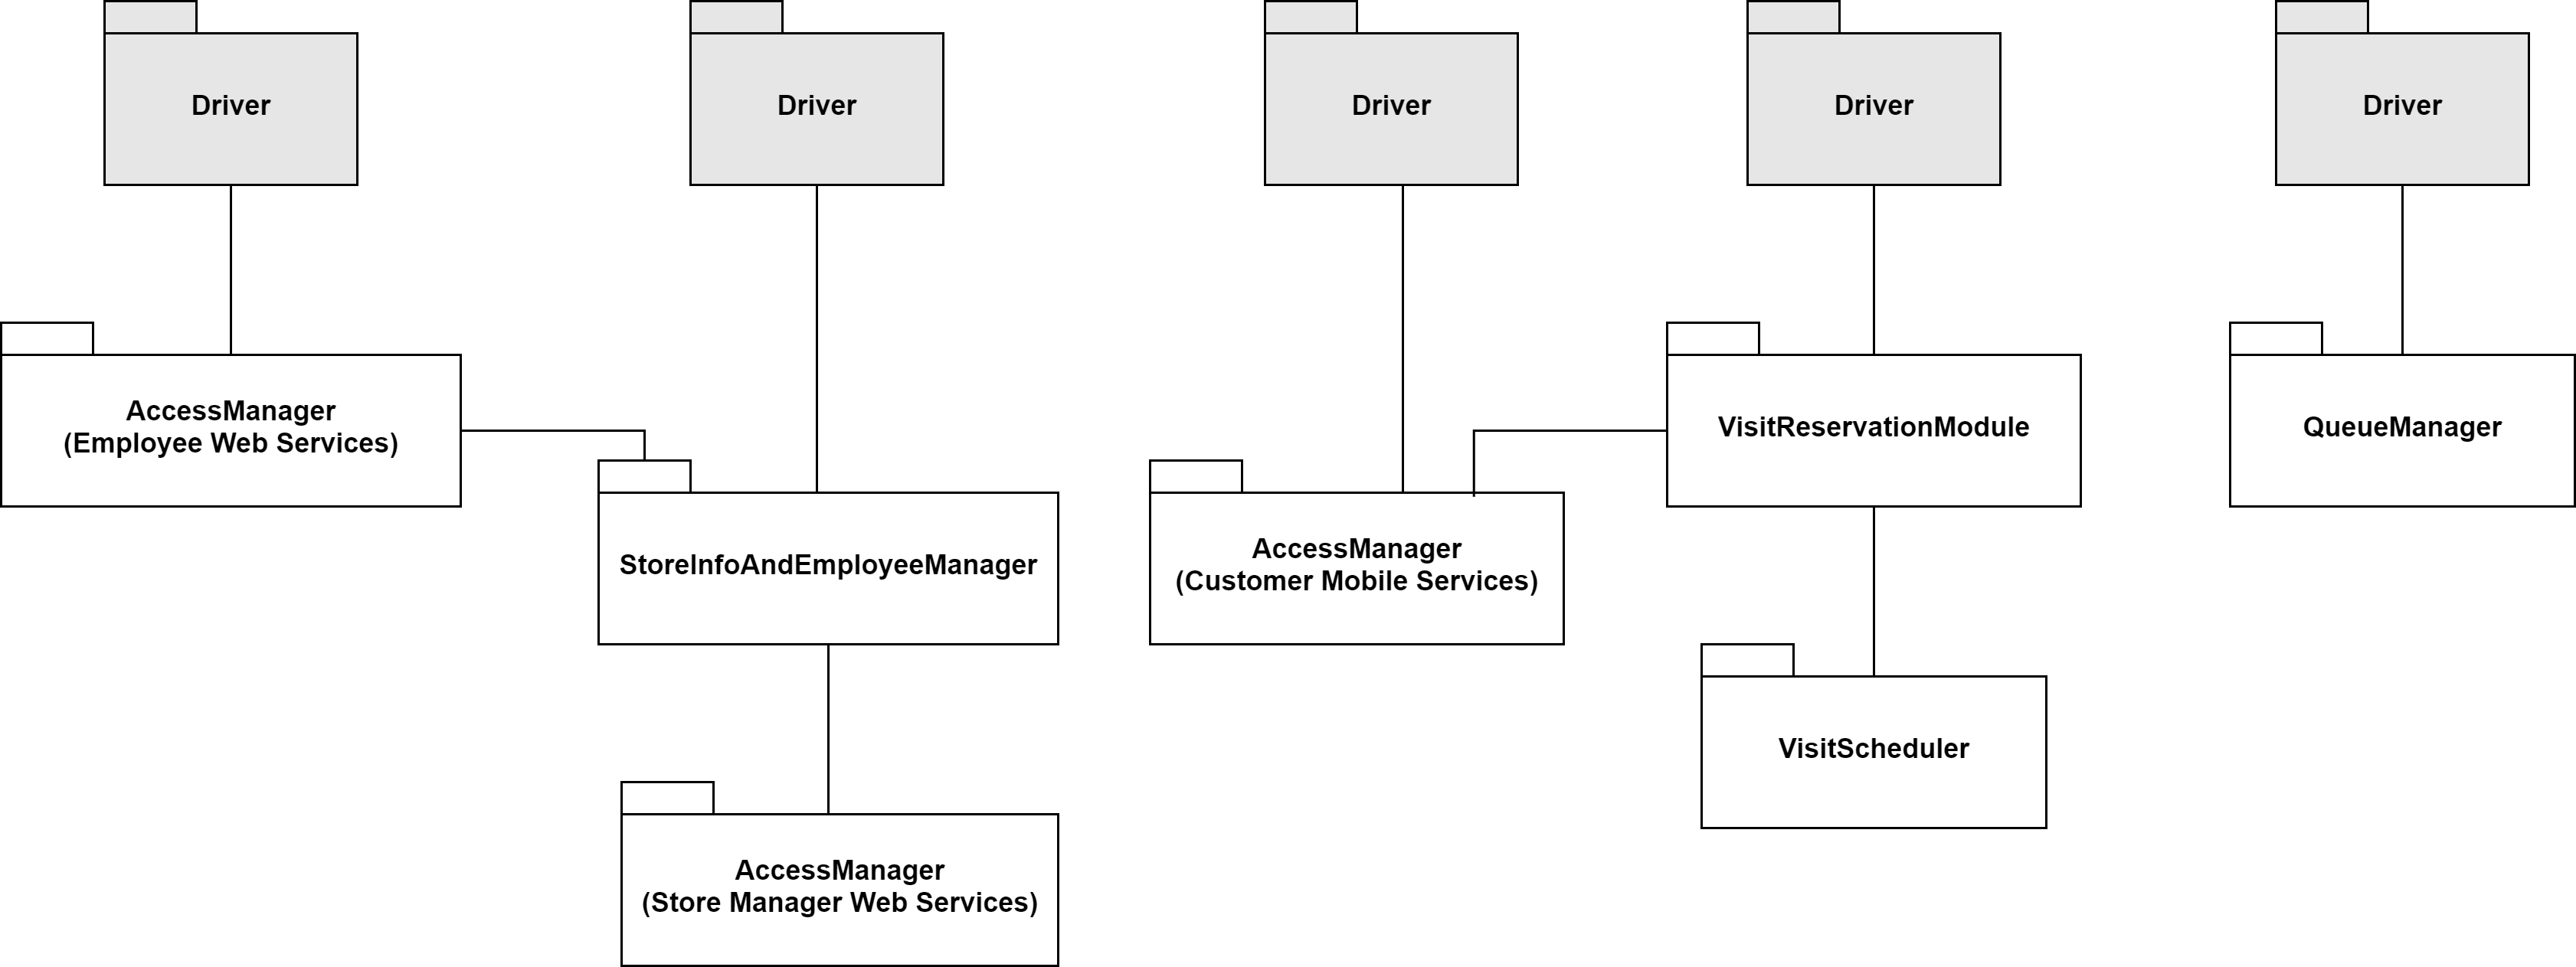
\includegraphics[width=12cm]{int_diagr6.png}
            \end{figure}
            \item \textbf{Employee and Customer Line Up Reservation Developing}: In this step it's necessary to implement and produce unit test for the component \textit{LineUpReservationModule} (Employee Web Services, Customer Mobile Services). As you can see in the diagram, the component in this stage has to be integrated and tested with \textit{QueueManager} and \textit{AccessManager} (Employee Web Services, Customer Mobile Services). Following the bottom-up approach it uses a Driver to represents the high level components to be developed \begin{figure}[H]
                \centering
                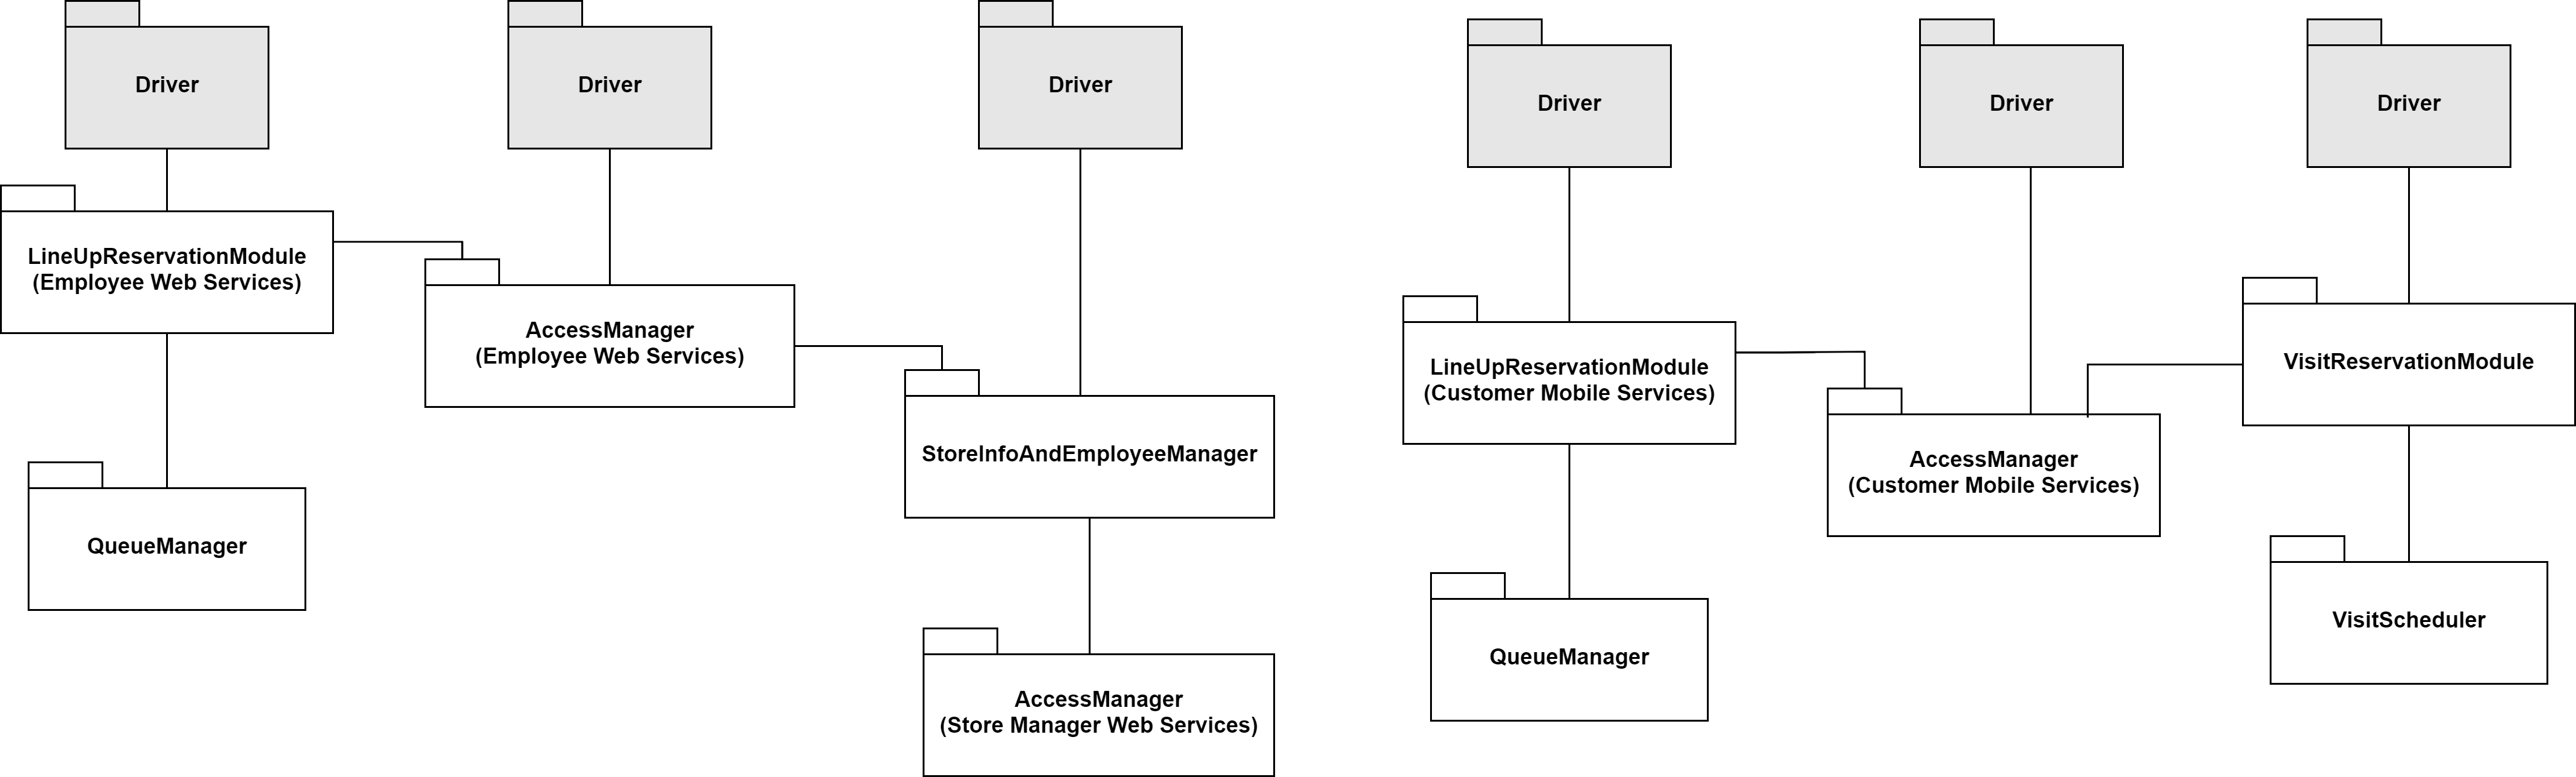
\includegraphics[width=\textwidth]{int_diagr7.png}
            \end{figure}
            \item \textbf{Entrances and Exits Developing}: In this step it's necessary to implement and produce unit test for the component \textit{EntrancesAndExitsModule}. As you can see in the diagram, the component in this stage has to be integrated and tested with \textit{AccessManager} (Employee Web Services). Following the bottom-up approach it uses a Driver to represents the high level components to be developed \begin{figure}[H]
                \centering
                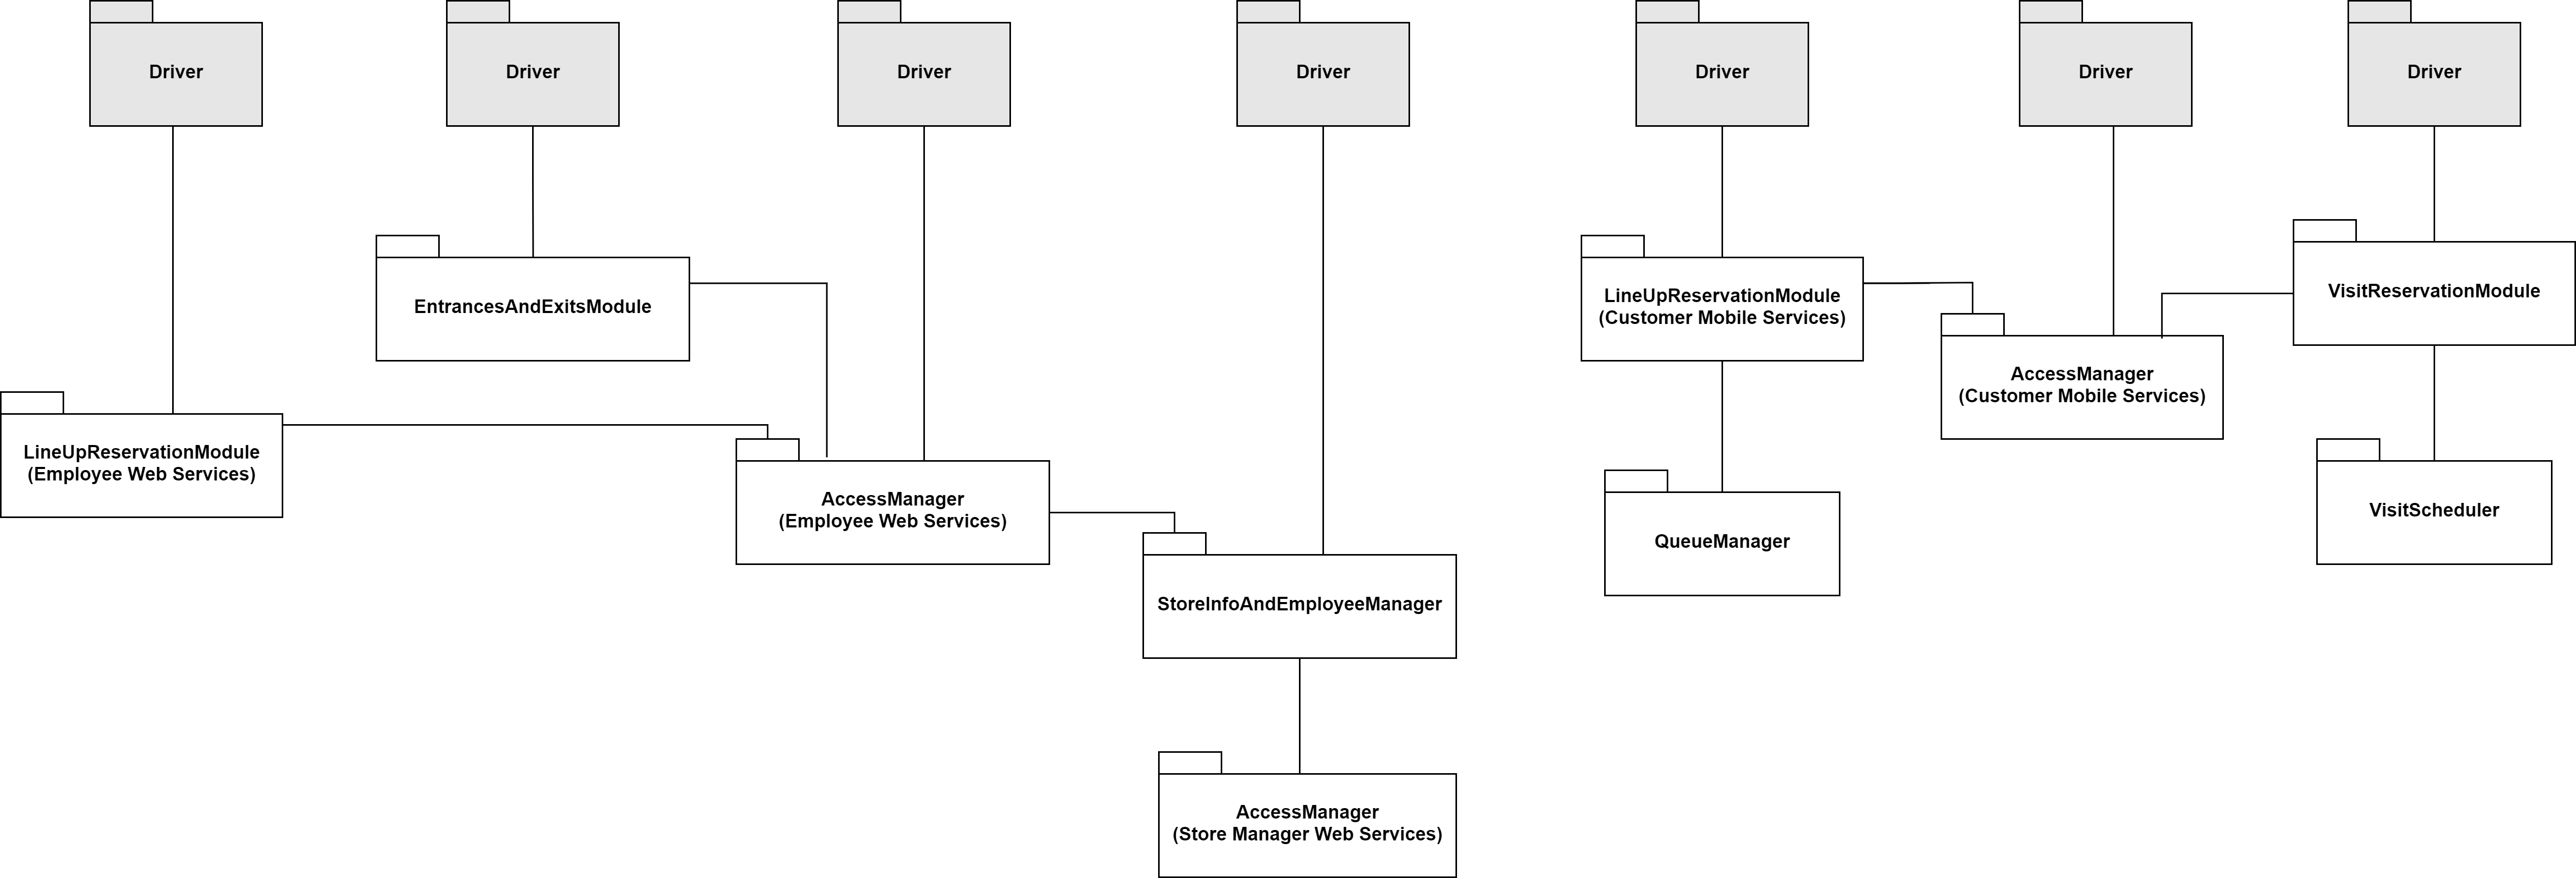
\includegraphics[width=\textwidth]{int_diagr8.png}
            \end{figure}
            \item \textbf{Data Analyzer Developing}: In this step it's necessary to implement and produce unit test for the component \textit{DataAnalyzer}. As you can see in the diagram, the component in this stage has to be integrated and tested with \textit{EntrancesAndExitsModule}. Following the bottom-up approach it uses a Driver to represents the high level components to be developed \begin{figure}[H]
                \centering
                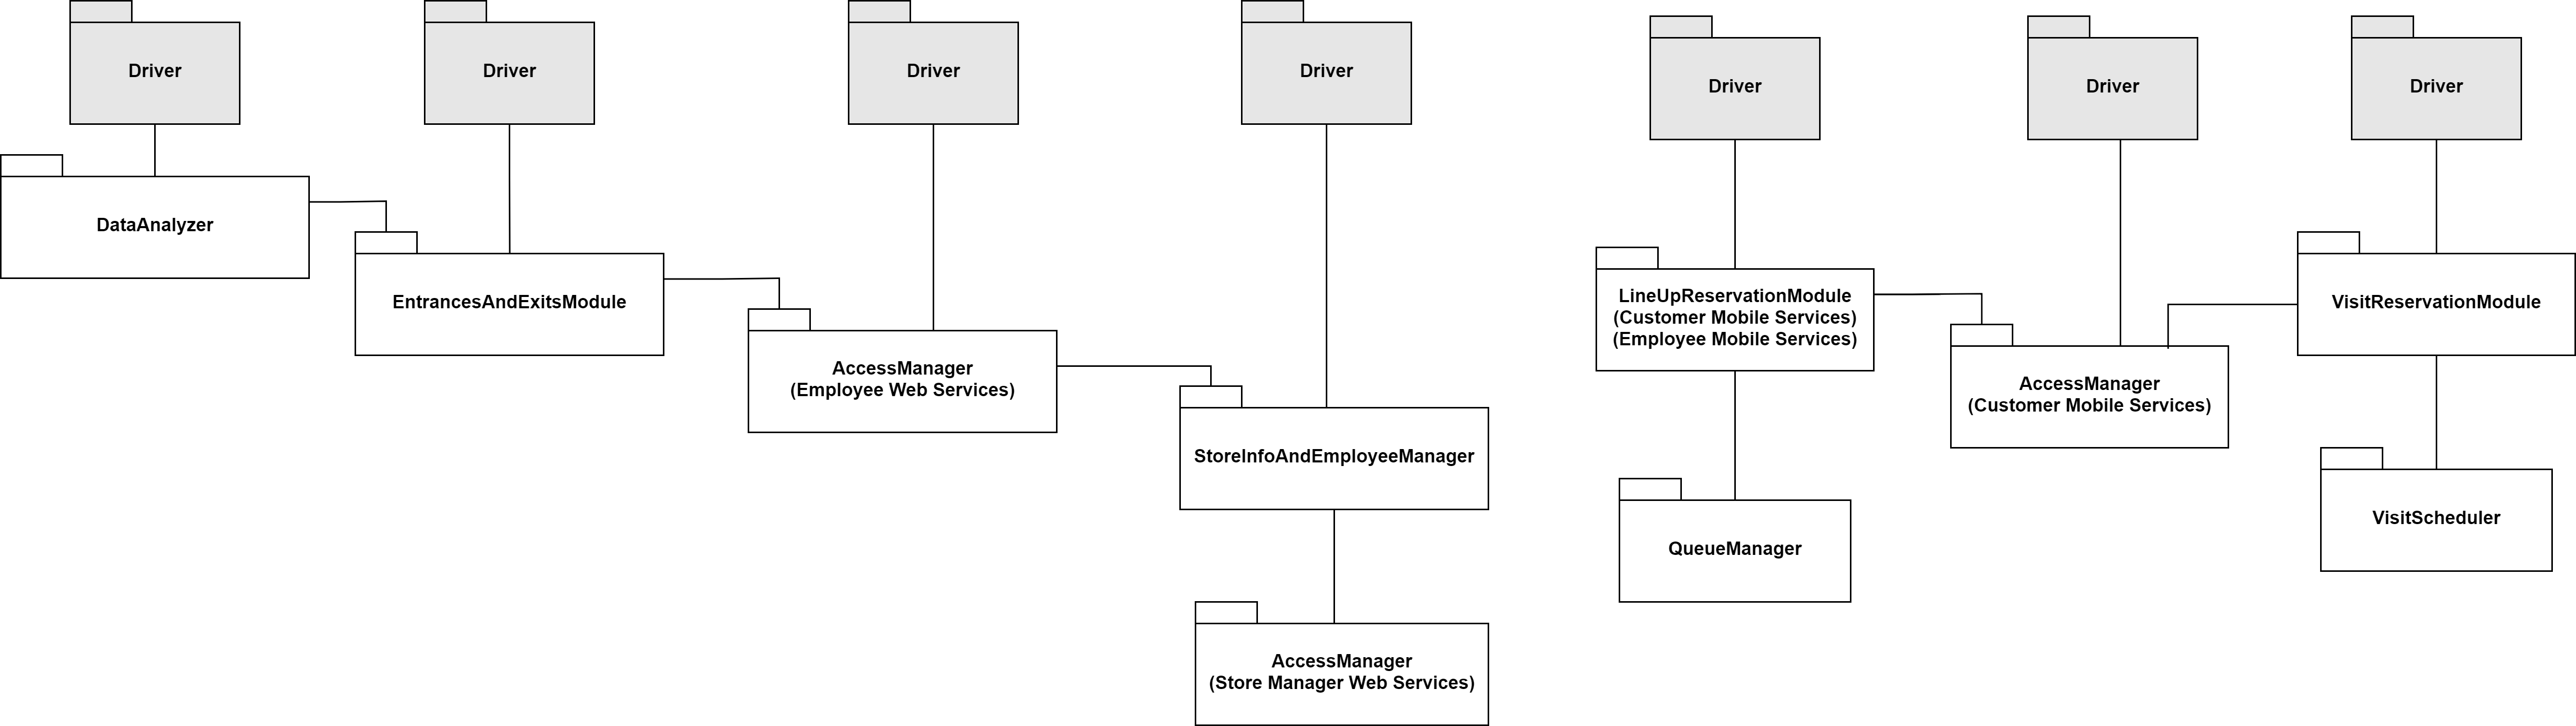
\includegraphics[width=\textwidth]{int_diagr9.png}
            \end{figure}
            \item \textbf{Statistics and Data Elaborator Developing}: In this step it's necessary to implement and produce unit test for the component \textit{StatisticsAndDataGateway}. As you can see in the diagram, the component in this stage has to be integrated and tested with \textit{DataAnalyzer}. This is the last step, so, following the bottom-up approach, the top level components take the place of the Drivers \begin{figure}[H]
                \centering
                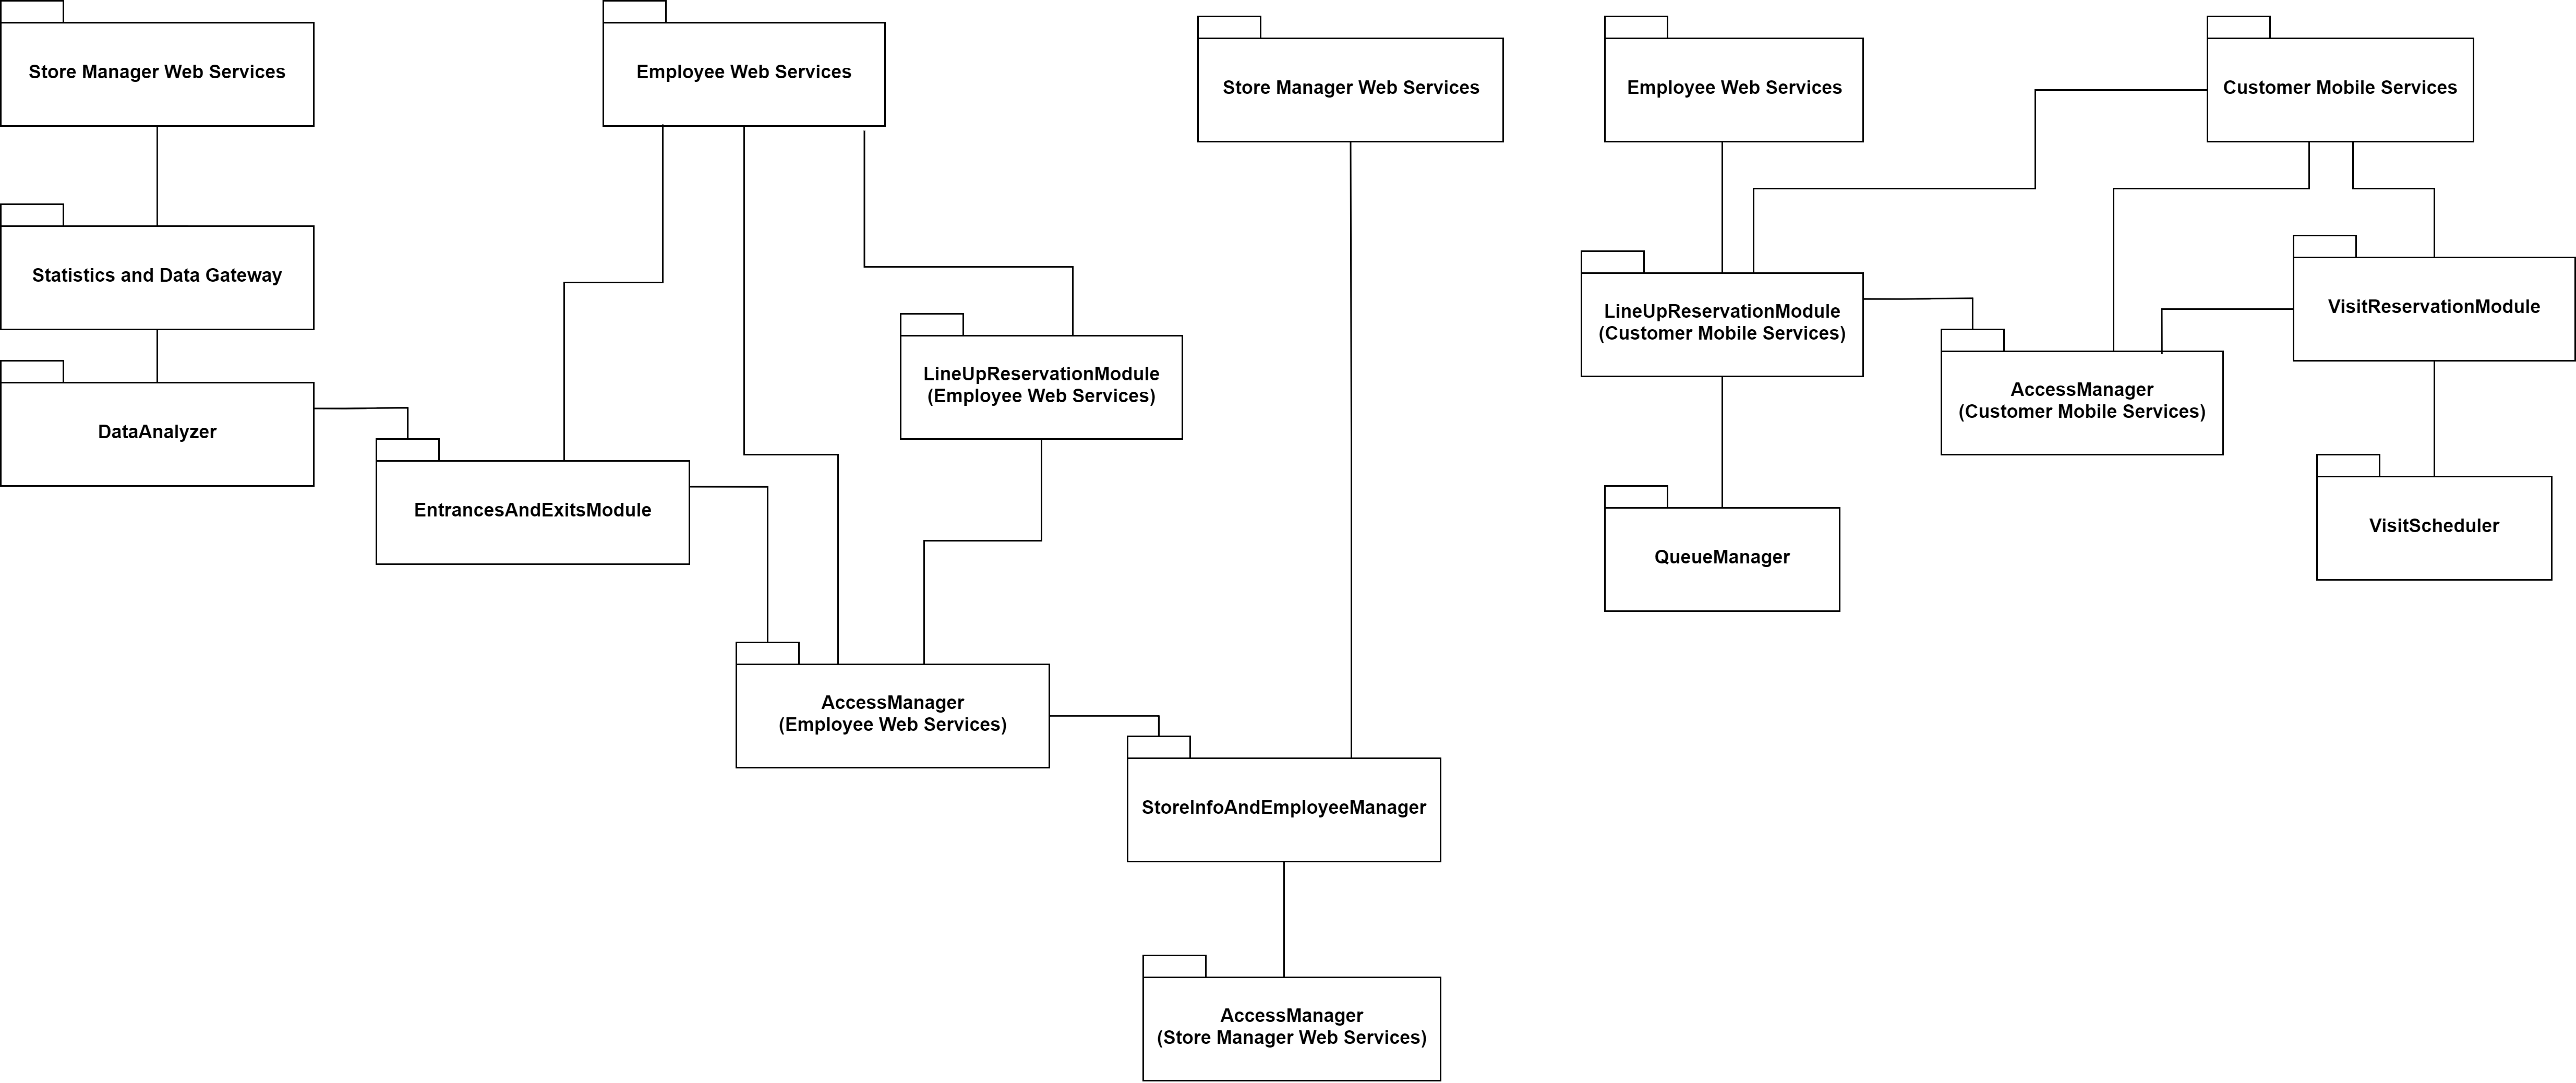
\includegraphics[width=\textwidth]{int_diagr10.png}
            \end{figure}
            \item \textbf{Client-Side and Server-Side Integration}: In this step, as previously anticipated, the Client-Side components and the Server-Side components have to be integrated. \begin{figure}[H]
                \centering
                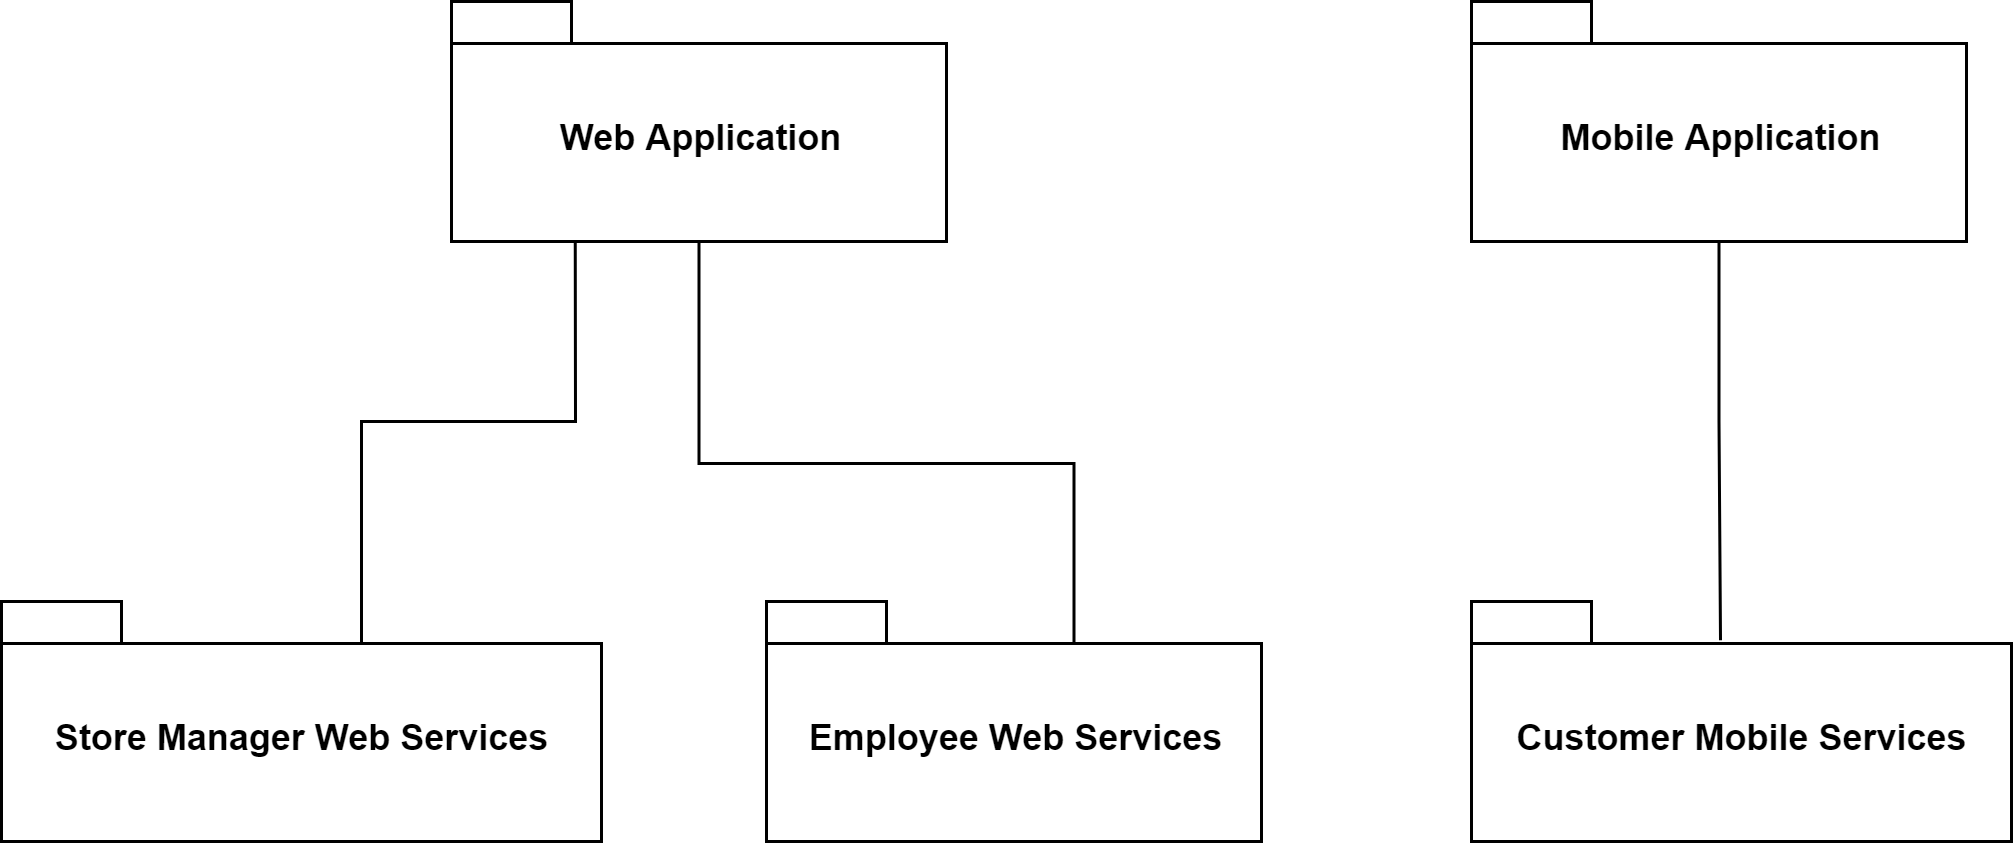
\includegraphics[width=8cm]{int_diagr11.png}
            \end{figure}
        \end{enumerate}
